\capitulo{3}{Conceptos teóricos}

\section{Anatomía del iris}
El iris se corresponde con la parte coloreada del ojo, se trata de un músculo circular(o elíptico) protegido por la córnea en cuyo centro se encuentra la pupila. Consta de 2 músculos el \emph{dilatador} y el \emph{esfínter} cuya función es ajustar el tamaño del iris para controlar la cantidad de luz que entra en la pupila.
El conjunto iris-pupila se encuentra rodeado por una membrana de color blanco llamada \emph{esclera}. Ver Figura \ref{fig:eye-anatomy}

El color, la textura y los patrones del iris son únicos y se cree que se forman aleatoriamente durante el periodo embrionario(etapa comprendida entre fecundación y la octava semana de embarazo), de modo que incluso 2 gemelos genéticamente iguales tienen distintos patrones.

En un entorno con mucha luz el esfínter contrae la pupila, dejando pasar menos luz a la retina, mientras que en un entorno poco iluminado, el músculo dilatador, dilata la pupila para permitir la entrada de más luz.
El ojo está protegido externamente por los párpados y las pestañas, sin embargo suponen un problema ya que pueden ocultar significativamente el iris y por tanto resultar en un mal reconocimiento.
%\begin{figure}[h]
%  \centering
%    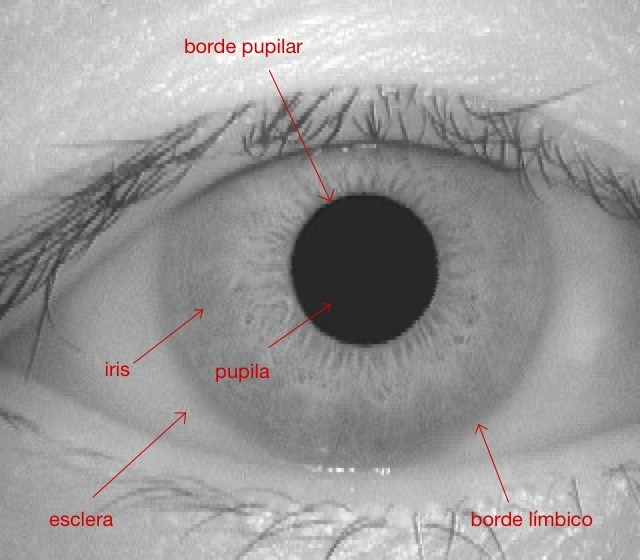
\includegraphics[width=0.7\textwidth]{eye-anatomy}
%  \caption{Imagen 001\_1\_1.bmp del dataset CASIA-Iris V1 que muestra las partes del ojo.}
%\end{figure}
%\newpage
\imagen{eye-anatomy}{Imagen 001\_1\_1.bmp del dataset CASIA-Iris V1 que muestra las partes del ojo.}
\section{Fases del reconocimiento}
Un sistema de reconocimiento tiene 3 fases:
\begin{enumerate}
	\item Adquisición de imágenes.
	\item Preprocesamiento de las imágenes:
	
	La cual se divide en 3 subfases:
	\begin{enumerate}
		\item Segmentación.
		\item Normalización.
		\item Extracción de \emph{features}(patrones del iris)
	\end{enumerate}
	\item Clasificación de las imágenes.

\end{enumerate}

\section{Adquisición de imágenes}
Es la primera de todas las fases y también la más trascendental ya que es necesario que las muestras tengan la calidad necesaria para que la posterior extracción de patrones sea eficiente.

Las muestras de un iris se toman con cámaras desarrolladas específicamente para este propósito si bien para este proyecto no se contaba con este hardware se podría haber optado por usar una cámara convencional(\emph{añadir referencia diabetes bachillerato}), pero ello incluiría otro problema: conseguir muestras de un gran número de voluntarios.
Para evitarse los problemas mencionados se optó por usar un dataset de iris, concretamente el de CASIA en su versión 1(\emph{añadir link a CASIA}) la cual está disponible de forma gratuita mediante registro y autorización previa.

Este dataset cuenta con 756 imágenes del iris de 108 sujetos. La toma de muestras se realizó en 2 sesiones, tomándose 3 muestras en la primera sesión y 4 en la segunda, de modo que se cuenta con un total de 7 muestras por sujeto.
Cada muestra está en formato \emph{.bmp} y tienen una resolución de 320x280.
Para la toma de muestras usaron una cámara desarrollada por la propia CASIA.
\imagen{casia-camera}{Toma de muestras para el dataset CASIA-Iris-V1}
Con el objetivo de facilitar la detección de los bordes del iris, las muestras se han editado, de modo que se han eliminado los reflejos especulares(\emph{añadir pie de página con definición}).

Cabe recalcar que dichas ediciones son mínimas y se aplican únicamente en la pupila, la cual no proporciona ninguna información útil para las etapas posteriores de extracción y clasificación de los patrones del iris.(\emph{añadir referferencia a image understanding for irsi.... }
\imagen{specular}{Imagen S1143R01.jpg perteneciente CASIA-Interval-V3 con regiones especulares(izquierda). Imagen 001\_1\_1.bmp de CASIA-Iris-V1 sin regiones especulares(derecha)}



\section{Listas de items}

Existen tres posibilidades:

\begin{itemize}
	\item primer item.
	\item segundo item.
\end{itemize}

\begin{enumerate}
	\item primer item.
	\item segundo item.
\end{enumerate}

\begin{description}
	\item[Primer item] más información sobre el primer item.
	\item[Segundo item] más información sobre el segundo item.
\end{description}
	
\begin{itemize}
\item 
\end{itemize}

\section{Tablas}

Igualmente se pueden usar los comandos específicos de \LaTeX o bien usar alguno de los comandos de la plantilla.

\tablaSmall{Herramientas y tecnologías utilizadas en cada parte del proyecto}{l c c c c}{herramientasportipodeuso}
{ \multicolumn{1}{l}{Herramientas} & App AngularJS & API REST & BD & Memoria \\}{ 
HTML5 & X & & &\\
CSS3 & X & & &\\
BOOTSTRAP & X & & &\\
JavaScript & X & & &\\
AngularJS & X & & &\\
Bower & X & & &\\
PHP & & X & &\\
Karma + Jasmine & X & & &\\
Slim framework & & X & &\\
Idiorm & & X & &\\
Composer & & X & &\\
JSON & X & X & &\\
PhpStorm & X & X & &\\
MySQL & & & X &\\
PhpMyAdmin & & & X &\\
Git + BitBucket & X & X & X & X\\
Mik\TeX{} & & & & X\\
\TeX{}Maker & & & & X\\
Astah & & & & X\\
Balsamiq Mockups & X & & &\\
VersionOne & X & X & X & X\\
} 
